
\documentclass[english,12pt,a4paper,pdftex]{article}
%% This package is required
%% Choose your school from arts, biz, chem, elec, eng, sci.
%% Choose the character encoding scheme used by your editor: utf8, latin1

\usepackage[elec,utf8]{aaltothesis} % this is the default in aaltothesis.sty
%% Use this if you run pdflatex and use jpg/pdf-format pictures.

\usepackage{graphicx}

%% Use the macros in this package to change how the hyperref package below 
%% typesets its hypertext -- hyperlink colour, font, etc. See the package
%% documentation. It also defines the \url macro, so use the package when 
%% not using the hyperref package.
%\usepackage{url}

%% Use this if you want to get links and nice output with pdflatex
\usepackage[pdfpagemode=None,colorlinks=true,urlcolor=red,%
linkcolor=blue,citecolor=black,pdfstartview=FitH]{hyperref}

%% Use this if you write hard core mathematics, these are usually needed
\usepackage{amsfonts,amssymb,amsbsy}  

%% Horizontal margins, DO NOT TOUCH!
\setlength{\hoffset}{-1in}
\setlength{\oddsidemargin}{35mm}
\setlength{\evensidemargin}{25mm}
\setlength{\textwidth}{15cm}
%% Vertical margins, DO NOT TOUCH!
\setlength{\voffset}{-1in}
\setlength{\headsep}{7mm}
\setlength{\headheight}{1em}
\setlength{\topmargin}{25mm-\headheight-\headsep}
\setlength{\textheight}{23cm}

%% Output starts here
\begin{document}
%% Change the school field to describe your school if the autimatically 
%% set name is wrong
% \university{aalto University}{aalto-Yliopisto}
% \school{School of Electrical Engineering}{SähköTekniikan korkeakoulu}

%% Vain kandityölle: Korjaa seuraavat vastaamaan koulutusohjelmaasi
%%
%% Only for B.Sc. thesis: Choose your degree programme. 
%\degreeprogram{Electronics and electrical engineering}%

%% Only for M.Sc. and Licentiate thesis: Choose your department,
%% professorship and professorship code. 
\department{Department of Signal Processing and Acoustics}%
{Signaalinkäsittelyn ja akustiikan laitos}
\professorship{Speech and Language Processing}{}
\code{S-89}

%% Choose one of these:
%\univdegree{BSc}
%\univdegree{MSc}
%% Added by Jose: For the non-finnish/swedish, the Lic degree is half of a PhD.
%\univdegree{Lic}
%% Add by Jose: For engineering exchange students (old plan, not Bolonia), PFC in Spain
%% IMPORTANT: FPr is only valid with English!!!
\univdegree{FPr}
%% Should be self explanatory...
\author{Jose Mariano Moreno Pimentel}

%% Your thesis title. If the title is very long and the latex 
%% does unsatisfactory job of breaking the lines, you will have to
%% break the lines yourself with \\ control character. 
%% Do not hyphenate titles.
\spanishtitle{Efectos del Ruido en un Sistema Estad\'istico de S\'intesis de Voz}
\thesistitle{Effects of Noise on a Speaker-Adaptive Statistical Speech Synthesis}{}

\place{Espoo}
%% For B.Sc. thesis use the date when you present your thesis. 
\date{02.04.2014}

%% B.Sc. or M.Sc. thesis supervisor 
%% Note the "\" after the comma. This forces the following space to be 
%% a normal interword space, not the space that starts a new sentence. 
\supervisor{Prof.\ Mikko Kurimo}{Prof.\ Mikko Kurimo}

%% B.Sc. or M.Sc. thesis advisors(s). 
%%
%% Note that there has been a change in the official EN translation
%% of the Finnish title ``ohjaaja'' which in the previous version (1.5) 
%% of this document was called ``instructor''. The recommended
%% translation is now ``advisor''.  
%% However, the LaTeX internal variable remains \instructor
%% as there is little point to change the variable name. 
%%
%\instructor{Prof. Pirjo Professori}{Prof. Pirjo Professori}
%\instructor{D.Sc.\ (Tech.) Olli Ohjaaja}{TkT Olli Ohjaaja}
\instructor{M.Sc.\ (Tech.) Reima Karhila}{DI Reima Karhila}

%% Aalto logo: syntax:
% \uselogo{aaltoRed|aaltoBlue|aaltoYellow|aaltoGray|aaltoGrayScale}{?|!|''}
%% Logo language is set to be the same as the document language.
\uselogo{aaltoBlue}{''}

%% Create the coverpage
\makecoverpage

%% Force new page so that English abstract starts from a new page
\newpage
%
%\begin{resumencastellano}[english]
En este proyecto se estudian los efectos de distintos tipos de ruido sobre un sistema estad\'istico de s\'intesis de voz adaptativo al locutor.

Los s\'istemas estad\'isticos de s\'intesis de voz se han vuelto bastante populares en los \'ultimos a\~nos gracias a su flexibilidad y bajos requ\'isitos de memoria en comparaci\'on con otros s\'istemas tales como los concatena
\end{resumencastellano}
%% English abstract, uncomment if you need one. 
%% 
%% Abstract keywords
\keywords{speech synthesis, synthetic speech, TTS, HMM, noise robust, TTS adaptation}
%% Abstract text
\begin{abstractpage}[english]
In this project we study the effects of noise on a speaker-adaptive HMM-based synthetic system based on the GlottHMM vocoder.
%
A comparison is made to system based on the STRAIGHT vocoder when the background noise is babble noise.
%
Both objective and subjective evaluation methods were conducted.
%
GlottHMM is found to be less robust against severe noise.
%
When the noise is less intrusive, the used objective measures gave contradictory results and no preference to either vocoder was shown in the listening tests.
%
In the preference of moderate noise levels, GlottHMM performs as well as the STRAIGHT vocoder. 
\end{abstractpage}
%% Note that 
%% if you are writting your master's thesis in English place the English
%% abstract first followed by the possible Finnish abstract

%% Preface
%\mysection{Esipuhe}
\mysection{Acknowledgments}

\vspace{5cm}
Otaniemi, 24.9.2013

\vspace{5mm}
{\hfill Jose M.\ Moreno \hspace{1cm}}

%% Force new page after preface
\newpage

%% Table of contents. 
\thesistableofcontents

\newpage
%% List of figures
\listoffigures

\newpage
%% List of tables
\listoftables

%% Symbols and abbreviations
\mysection{Symbols and Abbreviations}
\subsection*{Symbols}
\begin{tabular}{l l}
	$\lambda$		& Hidden Markov model\\
	$F_{0}$		& Fundamental frequency\\
	$\mathbf{O}$	& Observation sequence vector\\
	$P$			 	& Probability\\
	$\mathbf{Q}$	& State sequence vector
\end{tabular}

\subsection*{Abbreviations}
\begin{tabular}{l l}
	CMLLR		& Constrained Maximum-Likelihood Linear Regression\\
	CSMAPLR		& Constrained Structural Maximum A Posteriori Linear Regression\\
	EM 			& Expectation-Maximization\\
	FFT 		& Fast Fourier Transform\\
	HMM			& Hidden Markov Model\\
	HNR			& Harmonic-to-Noise Ratio\\
	LP			& Linear Prediction\\
	LPC 		& Linear Predictive Coding\\
	LSF			& Line Spectral Frequency\\
	LSP			& Line Spectral Pair\\
	MAP			& Maximum A Posteriori\\
	MBE			& Mixed multi-Band Excitation\\
	MLSA		& Mel Log Spectrum Approximation\\
	MFCC		& Mel-Frequency Cepstral Coefficient\\
	MOS			& Mean Opinion Score\\
	PSOLA		& Pitch-Synchronous OverLap-Add\\
	SAT			& Speaker-Adaptive Training\\
	SMAP 		& Structural Maximum A Posteriori\\
	STRAIGHT	& Speech Transformation and Representation using Adaptive \\
				& Interpolation of weiGHT spectrum\\
	TEMPO		& Time-domain Excitation extractor using Minimum Pertubatin\\
				& Operator\\
	TTS			& Text-To-Speech
\end{tabular}
%% Corrects the page numbering, there is no need to change these
\cleardoublepage
\storeinipagenumber
\pagenumbering{arabic}
\setcounter{page}{1}

\section{Introduction}
\label{intro}
\thispagestyle{empty}

Speech synthesis is not a recent ambition in mankind history. The earliest attempts to synthesize speech are only legends starring Gerbert d'Aurillac (died 1003 A.D.), also known as Pope Sylvester II. The pretended system used by him was a brazen head: a legendary automaton imitating the anatomy of a human head and capable to answer any question. Back in those days, the brazen heads were said to be owned by wizards. Following Pope Sylvester II, some important characters in mankind history  were reputed to have one of these heads, such as Albertus Magnus or Roger Bacon.

During the 18th century, Christian Kratzenstein, a German-born doctor, physicist and engineer working at the Russian Academy of Sciences, was able to built acoustics resonators similar to the human vocal tract. He activated the resonators with vibrating reeds producing the the five long vowels: /a/, /e/, /i/, /o/ and /u/.

Almost at the end of the 18th century, in 1791, Wolfgang von Kempelen presented his Acoustic-Mechanical Speech Machine \cite{vonKempelen}, which was able to produce single sounds and some combinations. During the first half of the 19th century, Charles Wheatstone built his improved and more complicated version of Kempelen's Acoustic-Mechanical Speech Machine, capable of producing vowels, almost all the consonants, sound combinations and even some words.	

In the late 1800's, Alexander Graham Bell also built a speaking machine and did some questionable experiments changing with his hands the vocal tract of his dog and making the dog bark in order to produce speech-like sounds \cite{Schroeder93}.


\section{History of Speech Synthesis}
\label{history_speech_synthesis}
Speech synthesis can be defined as the artificial generation of speech. Nowadays the process has been facilitated due to the improvements made during the last 70 years in computer technology, making the computer-based speech synthesis systems lead the way supported by their flexibility and their easier access compared to mechanical systems. However, after the first resonators built by Kratzenstein, the fist speaking machine was built and presented to the world in 1791, and was obviously mechanic.

\subsection{Acoustical-Mechanical Speech Machines}
The speech machine developed by von Kempelen incorporated models of the lips and the tong, enabling it to produce some consonants as well as vowels. Although Kratzenstein presented his resonators before von Kempelen his speech machine, von Kempelen started his work quite before, publishing a book where he described the studies made on human speech production and the experiments he made with his speech machine over 20 years of work \cite{vonKempelen}.  

The machine was composed by a pressure chamber, acting as lungs, a vibrating reeds in charge of the functions of the vocal cords and a leather tube that was manually manipulated in order to change its shape as the vocal tract does in an actual person, producing different vowel sounds. It had four separate constricted passages, controlled by the fingers, to generate consonants. Von Kempelen also included in his machine a model of the vocal tract with a hinged tongue and movable lips so as to create plosive sounds \cite{Schroeder93, LemmettyMSc, flanagan_1973_speech}. 



\begin{figure}[htb]
	\begin{center}
		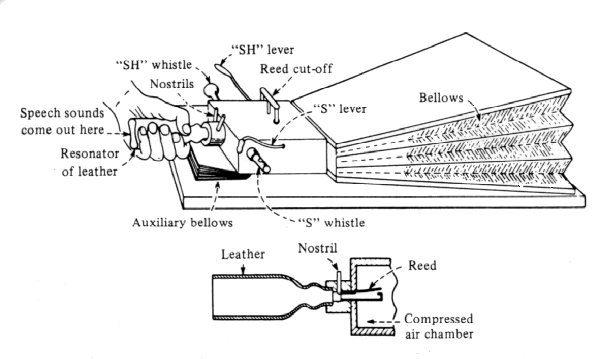
\includegraphics[width=\textwidth]{images/von_kempelen_machine.jpg}
		\caption{\cite{flanagan_book}}
	\end{center}
\end{figure}
\section{Speech Synthesis Systems}
\label{speec_synthesis_systems}
In this project we will use a HMM-based TTS system, but there are many different speech synthesis systems with their own advantages and disadvantages. In this section we will introduce the general architecture of a TTS system and diverse synthesis methods.

\subsection{TTS Architecture}
\label{speech_synthesis_systems_tts}
The main goal of a TTS system is to synthesize utterances from an arbitrary text. It is easy to notice that synthesizing from a text gives an extra flexibility to a synthesis system by allowing any reasonable input, in comparison to limited output systems such as GPS (Global Positional System) devices, but also an extra work has to be done to transform that text into the phonetic units required as inputs by the synthesizer. A general diagram of a TTS system is shown in Figure \ref{fig:tts_architecture}.

\begin{figure}[htb]
	\begin{center}
	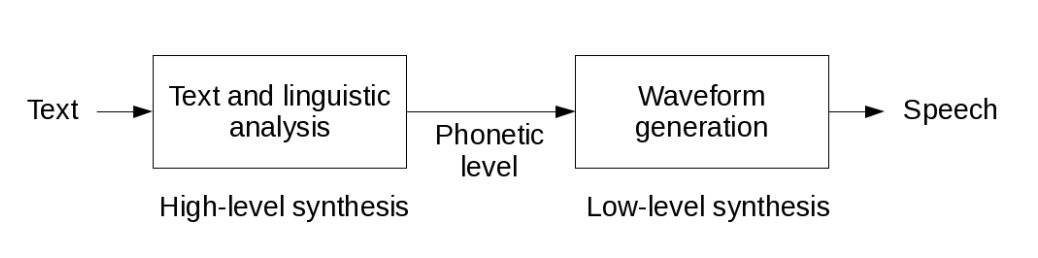
\includegraphics[width=\textwidth]{images/tts_architecture.jpg}
	\caption{General block diagram of a TTS system \cite{TuomoMSc}}
	\label{fig:tts_architecture}
	\end{center}
\end{figure}

The block representing the text and linguistic analysis is what differences a TTS system from other speech synthesis systems. The analysis made to the text has to generate the phonetic representation needed by the next component and predicting the desired prosody. Defining a larger set of goals for the speech synthesis system implies a more complex text and linguistic analysis. For example, trying to imitate the speaking style used by sports broadcaster in stead of synthesizing speech in a neutral style needs an extra function aiming to figure out the style of the input text, besides having constructed the corresponding model capable of producing speech mimicking the target style.

The main path followed by the text analysis includes a mandatory text normalization module. It is very important to normalize the text before trying to obtain its phonetic representation, to transform numbers, dates, acronyms and all the particularities that a language admit into a standardized form, called full-context labels representing the utterance on a phonetic-unit level based on the relations between phonemes, stress of each word, etc., accepted by the system. Also, this module is in charged of defining how similar spelled words are pronounced, e.g. the verb read has to different pronunciations whether is in the present tense or in the past tense. As it can be seen, text normalization is a complex problem that many researchers are looking for a solution to. An interesting approach to convert non-standard words (NSWs) into pronounceable words based on a taxonomy built from several text types is discussed in \cite{Sproat2001}.

Once the text is normalized, i.e. converted to plain letters, the structural properties of the text are analyzed and it is converted to a phonetic level. This last conversion is called the letter-to-sound conversion \cite{Pickett1999}. 

When the input text has gone through the first block represented in Figure \ref{fig:tts_architecture}, the low-level block generates predicts, based on the structural information and the prosodic analysis and tipically using statistical models, the fundamental frequency contour and phone durations. Finally, the speech waveform is generated by the vocoder. 

\subsection{Speech Synthesis Methods}
\label{speech_synthesis_systems_methods}
The generation of the waveform can be carried out in several ways, thus, we can talk about different speech synthesis methods. As written in \cite{TuomoMSc}, the different methods can be divided in two categories attending to whether the speech is generated from parameter, i.e. completely artificial, or real speech samples are used during the process. From all the methods explained in this section, only concatenative synthesis uses real samples to synthesize speech.

\subsubsection{Formant Synthesis}
\label{formant_speech_synthesis}
Formant synthesis is the most basic acoustic speech synthesis method. Based on the source-filter theory, which states that the speech signal can be represented in terms of source and filter characteristics \cite{Fant1970}, models the vocal tract with individually adjustable formant filters. The filters can be connected in serial, parallel or both. The different phonemes are generated by adjusting the center frequency, gain and bandwidth of each filter. Depending on the time intervals taken to do the adjustment, continuous speech can be generated. The source is modelled with voice pulses or noise.

Dennis Klatt's publication of the Klattalk synthesizer (see Section \ref{history_vocoder}) was the biggest boost received by formant synthesis. However, nowadays the quality given by this kind of synthesizers is lower than other newer methods, such as concatenative systems. Even so, formant synthesis is used in many applications such as reading machines for blind people, thanks to its intelligibility \cite{Pickett1999}.

\subsubsection{Articulatory Synthesis}
\label{articulatory_speech_synthesis}
The aim of articulatory synthesis is to model the human articulatory system as accurately as possible, using computational physical models. Therefore, this is theoretically the best method in order to achieve high-quality synthetic voices. However, modelling as accurately as possible raises the difficulty. The main setbacks are the difficult implementation needed in an articulatory speech synthesis system and the computational load, limiting this technique nowadays. Despite its currently limitations, articulatory models are being steadily developed and computational resources are still increasing, revealing a promising future.

\subsubsection{Concatenative Synthesis}
\label{concatenative_speech_synthesis}
Concatenative methods use prerecorded samples of real speech to generate the synthetic speech. It is easy to deduce that concatenative synthesis stands out from other methods of synthesis in terms of naturalness of individual segments. There are several unit lengths, such as word, syllable, phoneme, diphone, etc, that are smoothly combined to obtain the speech according to the input text. 

The main problem when using concatenative synthesis are the memory requirements. It is almost impossible to store all the necessary data for various speakers and contexts, making this technique the best one to imitate one specific speaker with one voice quality, but also makes it less flexible. It is difficult to implement adaptation techniques to obtain a different speaking style or a different speaker in concatenative speech. Apart from the storage problem, that thanks to the decrease in cost of digital storage and database techniques is becoming less serious, the discontinuities found in the joining points may cause some distortion even though the use of smoothing algorithms.

Concatenative systems may be the most widely used nowadays, but due to the limitations before commented, above all the flexibility problem, they might not be the best solution.

\subsubsection{LPC-Based Synthesis}
\label{lpc_based_speech_synthesis}
As in formant synthesis, in LPC-based synthesis utilizes source-filter theory of speech production. However, in this case the filter coefficients are estimated automatically from a short frame of speech, while in formant synthesis the different parameters are found for individual formant filters. Depending on the segment to be synthesized, the excitation needed is either a periodic signal, when synthesizing voiced segments, or noise, in case the segment is unvoiced. 

Linear Prediction (LP) has been applied in many different fields for a long time and was first used in speech analysis and synthesis in 1967. The idea is to predict a sample data by a linear combination of the previous samples. However, LPC targets not to predict any samples, but to represent the spectral envelope of the speech signal. 

Though the quality of basic LPC vocoder is consider poor, the more sophisticated LPC-based methods can produce high quality synthetic speech. The type of excitation is very important in LPC-based systems \cite{TuomoMSc}, but the strength of this method lays on its accuracy estimating the speech parameters and a relatively fast computational speed.

\subsubsection{HMM-Based Synthesis}
\label{hmm_based_speech_synthesis}
The use of HMMs in speech synthesis is becoming more popular. HMM-synthesis uses a statical model for describing speech parameters extracted from a speech database. Once the statistical models are built, they can be use to generate parameters according a text input that will be use for synthesizing. 

HMM-based synthesizers are able to produce different speaking styles, different speakers and even emotional speech. Other benefits are a smaller memory requirement and better adaptability. This last benefit is very interesting to us. While working with noisy data, limiting the amount of corrupted data used to train the system will probably affect positively to the quality of the synthetic speech obtained. Thus, constructing a high-quality average model and then taking profit of the adaptability of these systems to use the noisy data to train the adaptation transforms seems the correct approach. The data needed to train the adaptation transforms is always much lower than the training data used to built the average voice model.

On the other hand, naturalness is usually lower in HMM-based systems. But it must be said that these systems are improving very fast the quality of the synthetic speech obtained in terms of naturalness. 

As in this project we will be using HMM-based TTS systems, they are going to be described with more detail in Section \ref{hmm_synthesis}.

\section{HMM-Based Speech Synthesis}
\label{hmm_synthesis}
Statistical parametric speech synthesis has grown in the last decade thanks to the advantages commented in Section \ref{hmm_based_speech_synthesis}: adaptability and memory requirements. In this section HMM-Based Speech Synthesis and HMM-based systems are explained.

\subsection{Hidden Markov Models}
\label{hmm_syntheis_markov}
HMMs can be applied to modelling different kinds of sequential data.
%
They were first described in publications during the 1960s and the 1970s, but it was not until the 1980s when the theory of HMMs was widespread understood and started to be applied in speech recognition and synthesis.
%
Nowadays, HMMs are widely used along different fields and its popularity is still increasing.

As the name suggests, HMM-Based systems are statistical Markov models, where the systems modelled are assumed to be Markov processes, i.e. stochastic processes that satisfy the Markov property: the probability of a state transition depends only on the path of the past states.
%
The Markov property can be alternative described as a memoryless property: the next sample can be predicted from the current one, without using the past samples in the prediction.

Formally, HMMs are a doubly stochastic process formed by an underlying stochastic process that is not observable, i.e hidden, but can be observed through another set of stochastic processes that produce an observation sequence. 
%
Thus, the stochastic function of HMMs is a result of two processes, the underlying one is a hidden Markov chain with a finite number of states and the observable one consists on a set of random processes associated with each state.

An HMM can be defined as a finite state machine generating a sequence of time observations.
%
Each time observation is generated by deciding to which state to proceed in order to generate the observation according to the probability density function of the current state.
%
At any given discrete time instant, the process is assumed to be at some state.
%
The current state generates an observation according to its stochastic process and the underlying Markov chain changes states with time according to the state transition probability matrix. 
%
In principle, the order of the underlying Markov chain is not bounded.

In Figure \ref{fig:hmm_structure} a 6-state HMM structure in which at every time instant the state index can increase or stay the same, never decrease. 
%
A left-to-right structure is generally used for modelling systems whose properties evolve in a successive manner, as is the case of speech signal.

An N-state HMM is defined by a state transition probability distribution, an output probability distribution and an initial state probability distribution: $\mathbf{A} = \lbrace a_{ij}\rbrace _{i,j=1}^{N}$, $\mathbf{B} = \lbrace b_{j}(\mathbf{o})\rbrace _{j=1}^{N}$ and $\Pi = \lbrace \pi _{i} \rbrace _{i=1}^{N}$ respectively.
% 
$a_{ij}$ represents the state transition probability from state $q_{i}$ to state $q_{j}$ and $\mathbf{o}$ is the observation vector. A more compact notation the model is: $\lambda = (\mathbf{A},\mathbf{B},\Pi)$.

There are three main problems associated to HMMs:
\begin{enumerate}
	\item Finding an efficient way to calculate the probability of the observation sequence, $P(\mathbf{O}|\lambda)$, given an observation sequence $\mathbf{O} = (\mathbf{o}_{1},\mathbf{o}_{2},...,\mathbf{o}_{T})$ and a model $\Pi = \lbrace \pi _{i} \rbrace _{i=1}^{N}$
	\item How to choose an optimal state sequence $\mathbf{Q} = (q_{1},q_{2},...,q_{T})$ given the model and the observation sequence
	\item How to maximize $P(\mathbf{O}|\lambda)$ by adjusting the model parameters
\end{enumerate}

\begin{figure}[!htb]
\begin{centering}
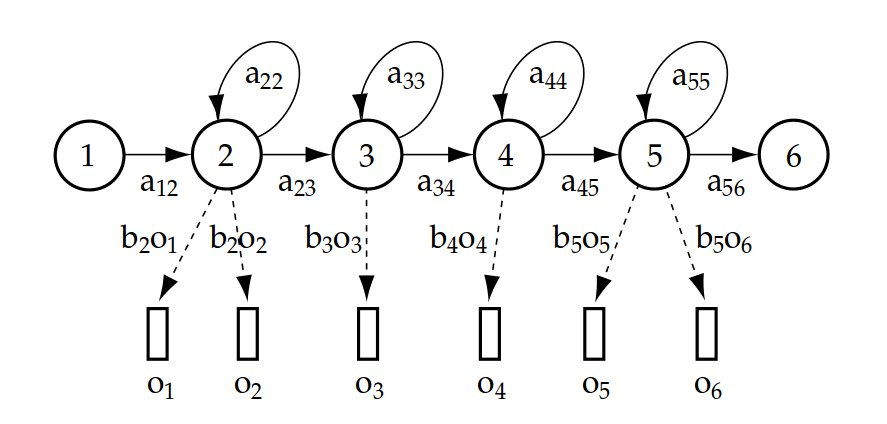
\includegraphics[width=0.7\textwidth]{images/hmm_structure.jpg}
\caption{6-state HMM structure. the states are denoted with numbered circles. State transitions probability form state $i$ to state $j$ are denoted by $a_{ij}$. Output probability densities of state $i$ are denoted $b_{i}$ and the observation generated at time instant $t$ is $o_{t}$}
\label{fig:hmm_structure}
\end{centering}
\end{figure}

Finding the probability that the observed sequence was produced by the given model causes the first problem, but it can be used to score different models based on how well they match the given observation sequence. This probability is calculated by the equation:

\begin{equation}
P(\mathbf{O}|\lambda) = \sum_{all \ Q} P(\mathbf{O}|\mathbf{Q},\lambda) \cdot P(\mathbf{Q}|\lambda)
\end{equation}

Although the calculation of $P(\mathbf{O}|\lambda)$ is straightforward, it involves on the order of $2 \cdot T \cdot N^{T}$ calculations, which is far from being efficient.
%
To reduce the computational cost of this calculation, this problem is usually evaluated with the Forward-Backward algorithm (see \cite{rabiner89}), requiring $N^{2} \cdot T $ calculations.

To solve the second problem we need to find the single best state sequence for a given observation sequence and a given model, i.e. we need to find $Q* = arg max_{Q} P(\mathbf{Q}|\mathbf{O},\lambda)$. 
%
This is usually solved using the Viterbi-algorithm \cite{viterbi67}. 

The third problem listed before is the most difficult one to solve.
%
Solving the model which maximizes the probability of the observation sequence has no known analytical solution. 
%
In stead, gradient based algorithms and iterative algorithms such as the Expectation-Maximization (EM) algorithm \cite{dempster77} are being used for maximizing $P(\mathbf{O}|\lambda)$.

HMMs have the possibility of being extended with various features, increasing the versatility and efficiency depending on the needs of the user. 
%
For example, state tying, state duration densities and inclusion of null transitions are among the extensions proposed.
%
More information about HMMs can be found in  \cite{rabiner89} and \cite{rabiner93}.

\subsection{HMM-Based Speech Synthesis System}
\label{hmm_synthesis_based_system}
In this project an HMM-based speaker-adaptive synthesis system will be used to synthesize speech with different speaker styles.
%
In \cite{tokuda13} a general overview of speech synthesis based in HMMs can be found.

\subsubsection{System Overview}
\label{hmm_synthesis_based_system_overview}
The general overview of a HMM-based synthesis system is ilustrated in Figure \ref{fig:hmm_system_overview}.

\begin{figure}[!htb]
\begin{centering}
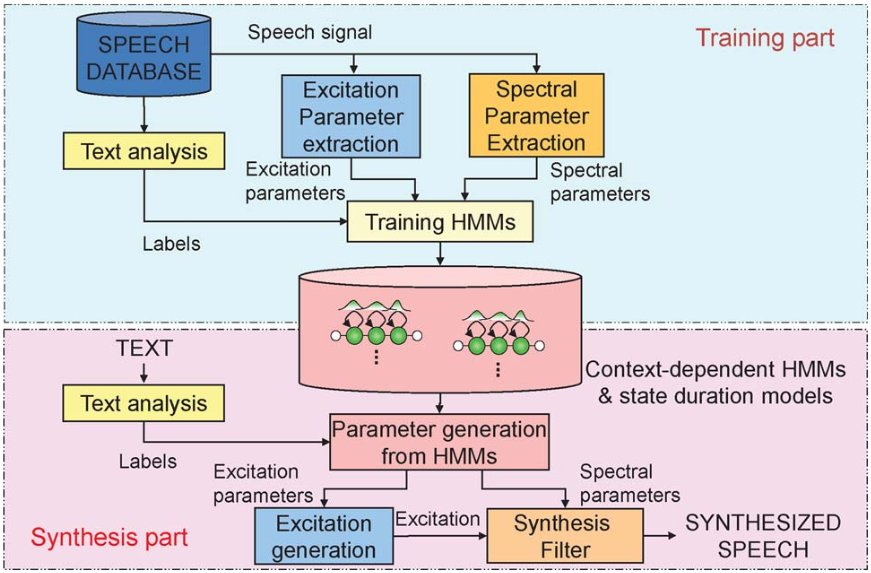
\includegraphics[width=\textwidth]{images/hmm_based_system_overview.jpg}
\caption{Overview of an HMM-based speech synthesis system \cite{tokuda13}}
\label{fig:hmm_system_overview}
\end{centering}
\end{figure}

An HMM-based system can be divided in two major parts: training and synthesis. 
%
In the training part, the vocoder extracts the speech parameters of every sample in the speech database and the labels containing the translation to the phonetic unit used, as explained in Section \ref{speech_synthesis_systems_tts}.
%
Then, the obtained parameters are modeled in the framework of the HMM.
%
The goal of the synthesis part is to produce a speech waveform according to the text input.
%
This process begins with the analysis of the text, as in the training part, in order to concatenate the required HMMs for that particular sentence and generate the parameters to feed the synthesis module and generate the speech waveform.

In this project we will be using a speaker-adaptive system. 
%
Thus, there is an extra part not represented in the general overview of an HMM-based system shown in Figure \ref{fig:hmm_system_overview}: adaptation. 
%
Before the parameter generation a transformation is applied to the context-dependent HMMs and the state duration models, aiming to convert them into models of the target speaker.
%
Adaptation makes synthesis with little data from a specific speaker possible, but it must be done from a good average voice model, built out from several speakers, and the differences between the average voice model and the target speaker will highly affect the similarity between the real speaker and the synthetic voice.
%
In Section \ref{hmm_synthesis_adaptation} an overview of a speaker-adaptive system is given and the adaptation technique used is explained.

The next sections explain the different steps that are done while constructing the HMM-based speech synthesis system.

\subsubsection{Speech Parametrization}
\label{hmm_synthesis_parametrization}
The first step of the training part is to extract from the speech signal a few parameters which function is to describe the essential characteristics of the speech signal as accurately as possible, compressing the original information.
%
A very efficient way was found in separating the speech signal to source and filter \cite{Fant1970}, both represented by coefficients. 
%
Both, STRAIGHT and GlottHMM follow the source-filter theory, although it is not the only approach to this problem, it is a functional trade-off between the accurate but complex direct physical modelling and a reasonable analytic solution.
%
This approach models the speech as a linear system where the ideal output is equivalent to the physical model, but the inner structure does not mimic the speech production physical structure.

In Section \ref{vocoders} the differences between the speech parametrization done by GlottHMM and STRAIGHT can be found, as they implement a different solution to this problem while following the same source-filter structure.

\subsubsection{Training of HMM}
\label{hmm_synthesis_training}
Once the parametrization is done, the speech features obtained are used to train a voice model. 
%
During the training, maximum-likelihood estimation of the HMM parameters is performed.

The case of speech synthesis is a particular one, as the $F_{0}$ values are not define in the unvoiced region, the observation sequence of $F_{0}$ is composed of 1-D continuous values and also discrete values or symbols representing the unvoiced.
%
HMMs need to model both the excitation and spectral parameters at the same time, but applying both the conventional discrete and continuous HMMs to model $F_{0}$ cannot be done directly. 
%
Thus, to model the $F_{0}$ observation sequence, HMM-based speech systems use multispace probability distributions \cite{tokuda2002multi}. 
%
Tipically, the multispace distribution consists of a continuous distribution for the voiced frames an a discrete one for the unvoiced. 
%
Switching according to the space label associated with each observation makes possible to model variable dimensional vector sequences, in our case, the $F_{0}$ observation sequence.
% 
To keep synchronization between the spectral and the excitation parameters, they are simultaneously modelled by separate streams in a multistream HMM, which uses different output probability distributions depending on the features.

As shown in Figure \ref{fig:hmm_system_overview}, the training takes into account the duration and context to model the different HMMs.
%
The duration modelling specifies for each HMM a state-duration probability distribution that are used to model the temporal structure of the speech in detriment of transition probabilities.

The context dependency of the HMMs is needed in speech synthesis to deal with the linguistic specifications.
%
Different linguistics contexts, such as tone, pitch accent or speech stress among others, are used by HMM-based speech synthesis to build the HMMs.
%
Spectral parameters are mainly affected by phoneme information, but prosodic and duration parameters are also affected by linguistic information. In \cite{tokuda13} some of the contexts used in English can be found.

Finally, it is important to note that there are too many contextual factors in relation with the amount of the speech data available. 
%
Increasing the speech data will increase the number of contextual factors and exponentially their combinations.
%
Hence, limited amount of data will limit the accuracy and robustness of the HMMs estimation.
%
To overcome this issue, tying techniques as state clustering and tying model parameters among several HMMs are used in order to obtain a more robust model parameters estimation.
%
It must be noticed that spectral, excitation and duration parameters are clustered separately as they have different context dependency.

Once the HMMs are estimated regarding the considerations explained, the training part is finished and a model is built.
%
If the model aims to reproduce one speaker, we would be talking about a speaker-dependent model.
%
However, a speaker-adaptive system as the one used in this project aims to synthesize different speakers from one model as starting point.
%
This model is called speaker-independent model, and the only difference with the speaker-dependent model so far in the HMM-based system construction is that the speech data is composed by several speakers to cover different speaker styles.
%
However, when using speaker-independent models aiming to adapt to different speakers, a technique called speaker-adaptive training (SAT) is used to generate an average voice model by normalizing interspeaker acoustic variation \cite{anastasakos1996, yamagishi2003training}.

\subsubsection{Adaptation}
\label{hmm_synthesis_adaptation}
Figure \ref{fig:hmm_system_overview} shows the overview of a general HMM-based speech synthesis system.
%
In order to build a speaker-adaptive system, there is a third part that must be added to the structure before the synthesis: adaptation.

As commented previously, HMM-based systems are quite flexible, resulting in a good quality adaptive systems.
%
Figure \ref{fig:hmm_system_adapt_overview} illustrates a HMM-based speaker-adaptive system, hence, it shows the basic structure of both systems compared in this project.

\begin{figure}[!htb]
\begin{centering}
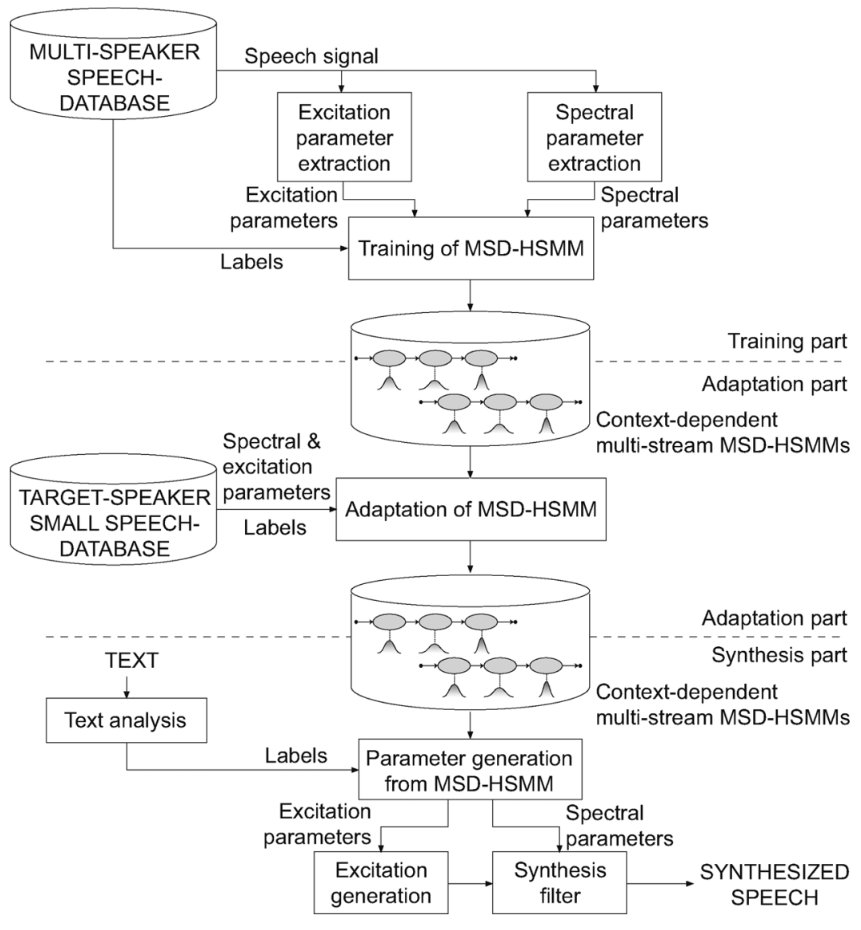
\includegraphics[width=0.8\textwidth]{images/hmm_based_system_adapt_overview.jpg}
\caption{Overview of an HMM-based speaker-adaptive speech synthesis system \cite{yamagishi2009}}
\label{fig:hmm_system_adapt_overview}
\end{centering}
\end{figure}

The adaptation layer between the training and the synthesis part is the only difference between the structures of an adaptive and a non-adaptive system.
%

Many adaptation techniques are used in HMM-based speaker-adaptive systems, all of them targeting the same: transforming an average voice model to match a predefined target using a very small amount of speech data.
%
Among the different targets we can find for example speaker adaptation or expressive speech.
%
In \cite{tokuda13} we can find several issues where adaptation techniques are helpful. 

Within the speaker-adaptive challenge, several techniques to approach a satisfying solution are available. 
%
\cite{yamagishi2009} proposes an adaptation algorithm called constrained structural maximum a posterior lineal regression (CSMAPLR) and compares several adaptation algorithms to figure out which one to use in which conditions.

The adaptations made during this project and in \cite{karhila_jstsp_14} use the CSMAPLR algorithm.
%
This algorithm combines different adaptation algorithms in a defined order. The algorithms used are:

\begin{itemize}
	\item Constrained maximum-likelihood liner regression (CMLLR)
	\item Maximum a posteriori (MAP)
	\item Structural maximum a posterior (SMAP)
\end{itemize}

When adapting in speech synthesis, it is important to adapt both the mean vectors and covariance matrices of the output and duration probability density functions, as the covariance is also an important factor affecting synthetic speech.
%
This is the reason to use CMLLR in stead of the unconstrained version.

The CMLLR adaptation algorithm uses the maximum-likelihood criterion \cite{digalakis1995speaker, gales1998maximum} to estimate the transforms. 
%
The criterion works well when large amount of data is available.
%
However, in the adaptation stage the amount of data is limited, a more robust criterion must be found: MAP.
%
The basis of MAP algorithm are explained in \cite{gauvain1994maximum} and an overview is given in \cite{yamagishi2009}.

In SMAP \cite{shinoda2001structural} the tree structures of the distributions effectively cope with the control of the hyperparameters.

\subsubsection{Synthesis}
\label{hmm_synthesis_synthesis}
The lower part of Figures \ref{fig:hmm_system_overview} and \ref{fig:hmm_system_adapt_overview} show the synthesis part of an HMM-based speech synthesis system.
%
The first step is to convert the given text into a sequence of context dependent labels.
%
Then, context-dependent HMMs are concatenated according to the labels calculated in the previous step, determining the duration of each state to maximize its probability based on its state duration probability distribution.
%
Once the original sentence has been translated to context-dependent HMMs, a sequence of speech parameters is generated and using both the spectral and excitation parameters the speech waveform is produced by the correspondent vocoder. 
\section{Vocoders}
\label{vocoders}
The interface with both the natural speech and the synthesized speech is the vocoder. In this section, the fundamentals of the vocoder are presented and a detailed description of the two vocoders compared in this project is given.

\subsection{Vocoder}
\label{vocoders_vocoder}
The human speech is produced by regulating the air from the lungs through the 
%\section{Introduction}

%% Leave first page empty
%\thispagestyle{empty}

%% In a thesis, every section starts a new page, hence \clearpage
%\clearpage



%% Three levels of hierarchy in sectioning should be enough

\clearpage

%% The \phantomsection command is nessesary for hyperref to jump to the 
%% correct page, in other words it puts a hyper marker on the page.

\phantomsection
%\addcontentsline{toc}{section}{Viitteet}
\addcontentsline{toc}{section}{References}
\bibliographystyle{ieeetr}
\bibliography{sections/references}



\appendix 
\clearpage
%% Adds the word "Appendices" to the table of contents
\addtocontents{toc}{\protect\contentsline{section}{Appendices}{}{appendix}}

 %% appendix example (starts with section) in Finnish

%% Equations, tables and figures have their own numbering in Appendices, REMEMBER TO DO EVERY TIME YOU START AN APPENDIX, THE LETTER A IS THE APPENDIX INDEX
\renewcommand{\theequation}{A\arabic{equation}}
\setcounter{equation}{0}  
\renewcommand{\thefigure}{A\arabic{figure}}
\setcounter{figure}{0}
\renewcommand{\thetable}{A\arabic{table}}
\setcounter{table}{0}


\end{document}
